Die Trusted Execution Environment (TEE) zeichnet sich durch drei wesentliche Eigenschaften aus, die ihre Funktionalität und Sicherheit beschreiben. 
Sie gewährleistet (1) die Authentizität des ausgeführten Codes, indem sie sicherstellt, dass dieser tatsächlich von der beabsichtigten Quelle stammt und nicht manipuliert wurde. 
Ein wichtiger Aspekt dabei ist die Möglichkeit der Remote Attestation. Diese erlaubt es, die Authentizität des Codes aus der Ferne zu verifizieren. 
Die TEE sichert (2) die Integrität des Codes, indem sie während der Ausführung sicherstellt, dass dieser nicht verändert wurde. Außerdem schützt sie (3) die Vertraulichkeit von Code, Daten und Laufzeitvariablen, indem sie sicherstellt, dass diese nur von privilegierten Parteien eingesehen werden kann\cite{Trusted}.

Aufgrund der Interaktion von Programmen innerhalb der TEE und Programmen außerhalb, kann die TEE auch als Kompartiment betrachtet werden. Diese Struktur ermöglicht eine klare Trennung zwischen den unterschiedlichen Kompartiments und ermöglicht so eine bessere Kontrolle über den Zugriff.

\subsection{TEE}
Der genaue Aufbau und das Verhalten von Trusted Execution Environments (TEEs) variieren, lassen sich aber, wie in Abbildung \ref{fig:TEE} zu sehen ist, im Allgemeinen in zwei Kategorien einteilen: (1) den Single-World-TEEs, die sich einen Adressraum mit dem unprivilegierten Host teilen, und (2) den Two-Worlds-TEEs, bei denen die CPU konzeptionell in eine normale und eine sichere Welt unterteilt ist\cite{TEEPaper}.

\begin{figure}[h]
    \centering
    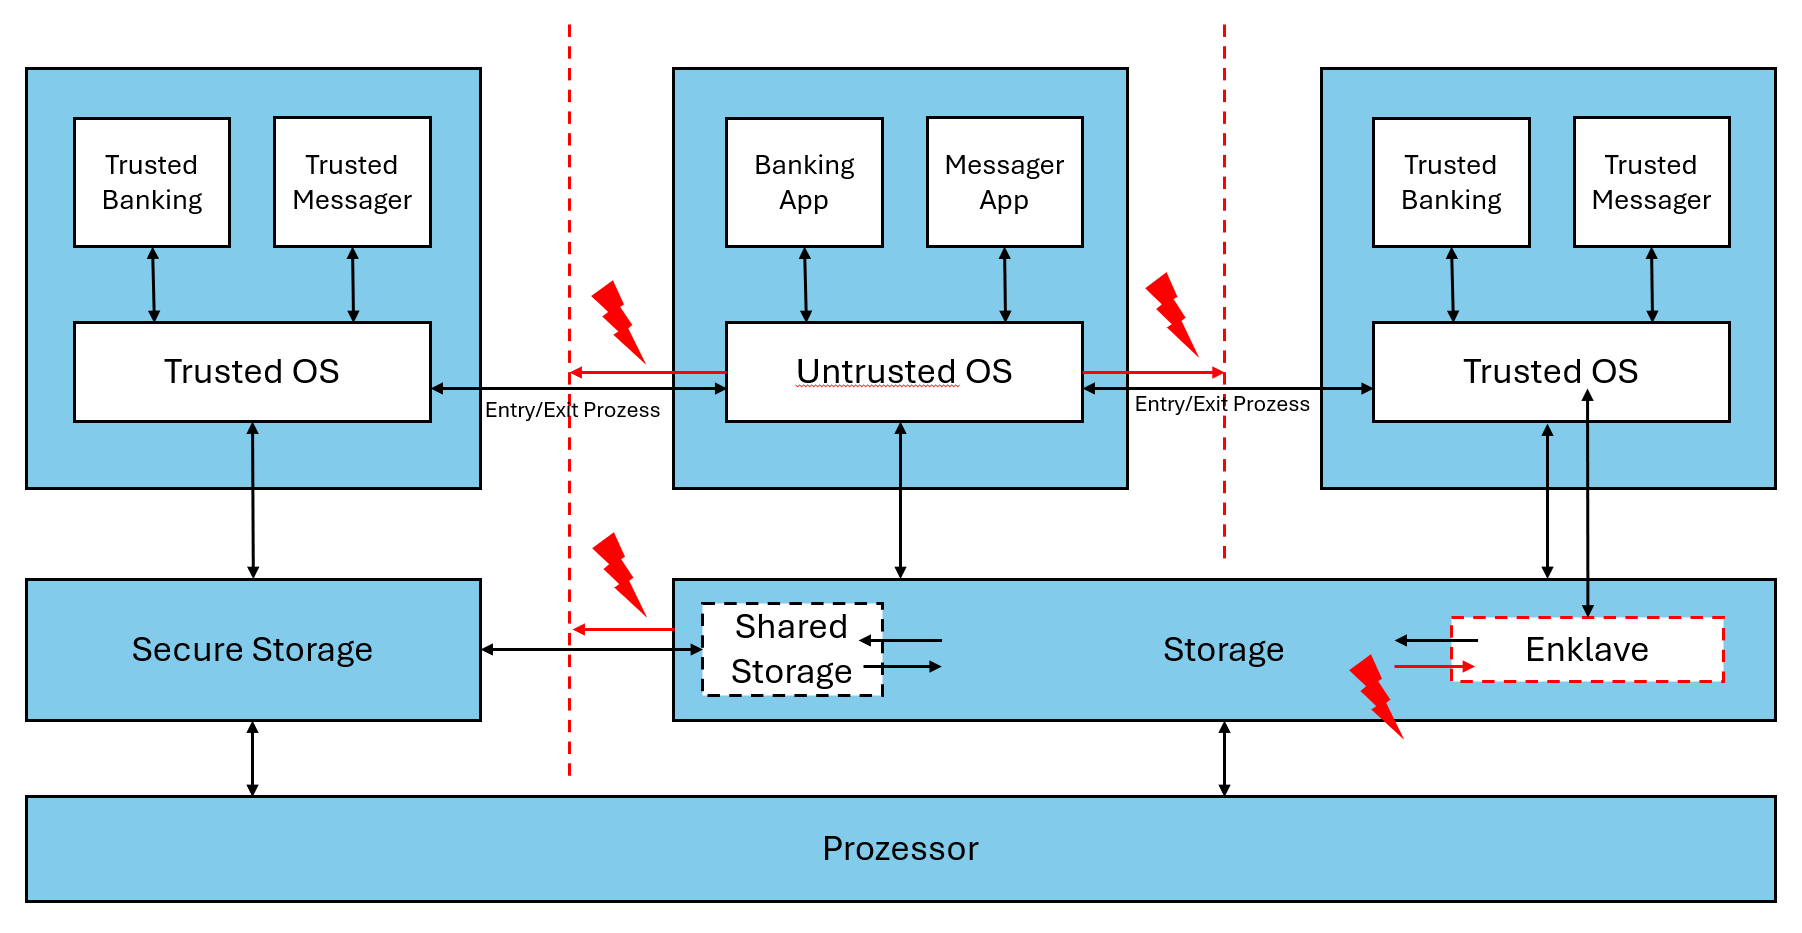
\includegraphics[width=\linewidth]{Grafiken/TEE-Grafik.png}
    \caption{Links der Aufbau einer TEE mit seperatem Adressraum, rechts eine TEE mit geteilten Adressraum in Form einer Enklave im Adressraum des unseren Host.}
    \label{fig:TEE}
\end{figure}

In der ersten Kategorie hat nur die Enklave selbst vollen Zugriff auf ihren Speicherplatz und kann die Daten im Klartext lesen. 
Eine Enklave ist ein isolierter Speicherbereich innerhalb einer TEE, der dazu dient, Code und Daten vor unautorisiertem Zugriff und Manipulation zu schützen.
Selbst privilegierte Benutzer und das Betriebssystem haben keinen Zugriff auf die innerhalb der Enklave gespeicherten Daten. 
Programme innerhalb der Enklave dürfen jedoch auch auf den Adressraum außerhalb der Enklave zugreifen. 
Diese Struktur ermöglicht einen besseren Datenaustausch, birgt jedoch das Risiko unsicherer Speicherzugriffe auf die möglicherweise korrupten Daten, was potenziell zu Sicherheitslücken führen kann.

In der zweiten Kategorie ist der Adressraum strikt in zwei separate Bereiche unterteilt, wobei keiner der beiden Bereiche auf den jeweils anderen zugreifen kann. 
Der Datenaustausch zwischen diesen beiden Welten erfolgt über das Trusted Operating System (TOS). 
Da das TOS privilegierten Zugriff hat, kann es einen geteilten Adressraum einrichten, in dem Daten sicher ausgetauscht werden können. 
Diese Methode bietet eine stärkere Isolation und somit ein höheres Maß an Sicherheit, da direkte Speicherzugriffe zwischen der normalen und der sicheren Welt verhindert werden, jedoch auf Kosten der Datenübertragungsraten.

In beiden Kategorien gewährleistet sowohl der Prozessor, dass extern kein Zugriff auf die Daten möglich ist, als auch das TOS, dass der Code in der Enklave sicher ist. Das TOS übernimmt außerdem den Entry/Exit Prozess der TEE, in dem der Übergang zwischen der normalen und der sicheren Welt ausgeführt wird. 

Neben den Angriffen auf das Application Binary Interface (ABI), welche auf Schwachstellen beim Erstellen und verlassen der TEE abzielen, gibt es noch das Application Programming Interface (API), welche versuchen Sicherheitslücken während der Laufzeit zu nutzen\cite{TEEPaper}.

Ein weiterer Grundgedanke beim Designen einer TEE ist Angreifer Model. Man entwickelt die TEE unter der Annahme, dass sie in einem System ausgeführt wird, das als kompromittiert betrachtet wird und Angreifer die volle Kontrolle über sämtliche Hardware haben.


\subsection{Kompartimentierung}

Die Kompartimentierung ist ein Konzept, das darauf abzielt, ein Computersystem oder einzelne Anwendungen in separate Bereiche aufzuteilen und diese möglichst isoliert voneinander operieren zu lassen. Diese Praxis beruht auf den Prinzipien der Sandbox und der Safebox, die eine sicherere und stabilere Systemumgebung ermöglichen\cite{CIVPaper}. Ein Kompartiment agiert als Safebox und behandelt alle anderen Programme als Sandbox und erlaubt kein Zugriff auf die eigenen Daten.

Eine Sandbox ist, wie in Abbildung \ref{fig:Sandbox} dargestellt, eine isolierte Ausführungsumgebung, in der ein Programm ausgeführt wird, welches keinen Zugriff auf Daten anderer Programme hat. 
Dies gewährleistet nicht nur die Sicherheit sensibler Informationen, sondern verhindert auch die Übernahme von Daten oder die Beeinflussung des Programmes durch potenziell kompromittierte Softwareteile. 
Ein bekanntes Beispiel dafür wäre eine Virtuelle Maschine (VM). Diese wird in einer isolierten Umgebung ausgeführt und hat kein Zugriff auf jegliche Daten außerhalb der Sandbox.
\begin{figure}[h]
    \centering
    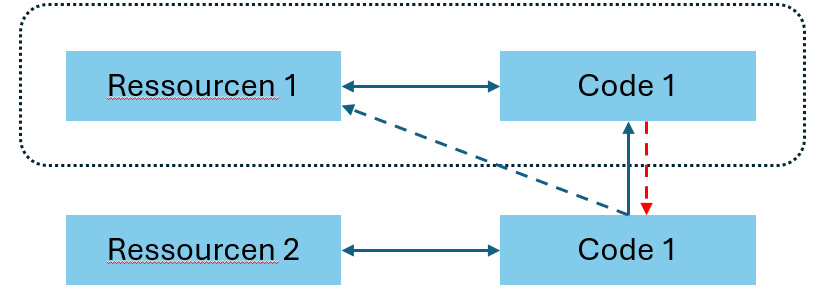
\includegraphics[width=0.8\linewidth]{Grafiken/Sandbox.png}
    \caption{Aufbau einer Sandbox.}
    \label{fig:Sandbox}
\end{figure}


Im Gegensatz dazu dient die Safebox, in Figure \ref{fig:Safebox} dargestellt, dem Schutz der eignen Daten. Dies wird ermöglicht, indem nur privilegierten Prozessen Zugriff auf die Daten gestattet wird. Diese Zugangskontrolle verhindert den Zugriff auf Daten eines anderen Kompartiments. 
Das ist genau die Funktionsweise einer Enklave. Die Programme innerhalb haben den vollen Zugriff, auch nach außen, aber die Daten sind von draußen nicht lesbar. \begin{figure}[h]
    \centering
    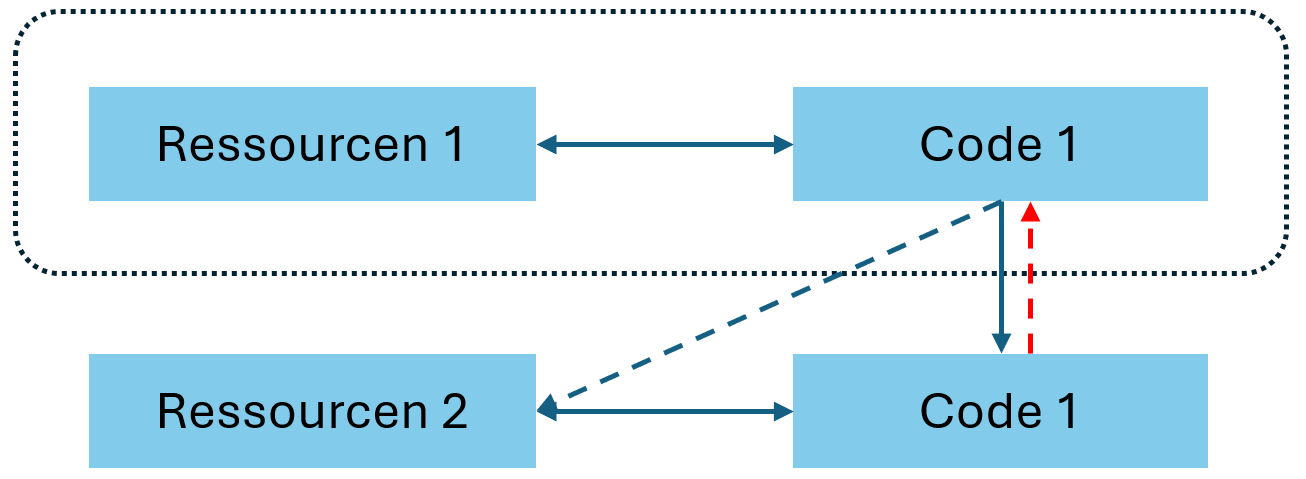
\includegraphics[width=0.8\linewidth]{Grafiken/Safebox.png}
    \caption{Aufbau einer Safebox.}
    \label{fig:Safebox}
\end{figure}

Das Initialisieren eines Kompartments lässt sich in 3 Stufen unterteilen. Zunächst erfolgt die Identifizierung, wo das Programm logisch gut unterteilt werden kann und wie feingranular diese Unterteilung sein soll.
Anschließend wird die Durchsetzung der Grenzen vorgenommen, indem die Programme logisch voneinander getrennt und ausschließlich über eine API zur Kommunikation zugelassen werden. 
In der letzten Stufe werden diese Grenzen weiter verhärtet. Hierbei wird die API-Schnittstellen weiter definiert, wie z.B. die Return Values und Pointer.

Wie in Figure \ref{fig:Kompartment} dargestellt, können Applikatonen in verschiedenen Kompartimenten nur über eine wohldefinierte API untereinander Daten austauschen.

\begin{figure}[h]
    \centering
    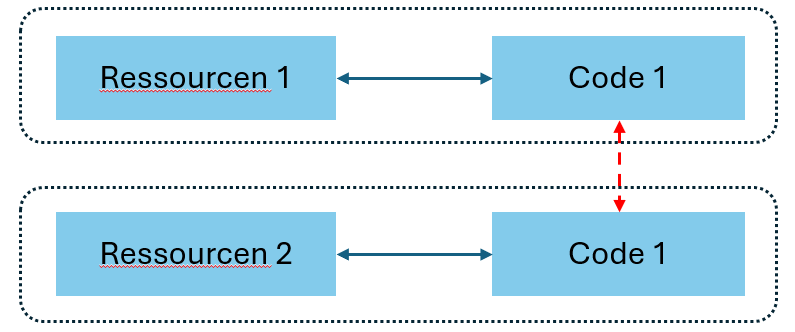
\includegraphics[width=0.8\linewidth]{Grafiken/Kompartiment.png}
    \caption{Aufbau von Kompartimenten}
    \label{fig:Kompartment}
\end{figure}

